\chapter{Newtons Laws and Kinematics}

\textbf{\textit{Note: }}Vector calculus cannot be applied to angles!!
Vector calculus can be applied to positions, linear velocities and accelerations, angular velocity and angular acceleration but not on angles!!

Because angles do not add up like any vector. To add up angles we need to use DCM's (Direction cosine matrix).

\section{Method for solving Dynamics Problem}

\begin{itemize}
	\item state the problem
	\item Draw figures including FBD's
	\item Describe motion
	\begin{itemize}
		\item determine degrees of freedom
		\item from DOF, define the coordinates of the motion problem
		\item also from DOF, equations of motion can be described for each of the DOF
	\end{itemize}
	\item assign the coordinates (generalized coordinates)
	\begin{itemize}
		\item match generalized coordinates
		\item match generalized velocities
	\end{itemize}
	\item explain correct physical laws
	\item do the math
\end{itemize}

\section{Derivative Rule from vector geometry}

Consider figure \ref{Fig_ch_0_01_DerivateRule}, in which there are tow points $A$ and $B$ which can be located from a reference point $O$ in an arbitrary reference frame $F$. The three position vectors can be drawn from $O$ which are labeled using vectors $r_{i/o}$ as shown in figure \ref{Fig_ch_0_01_DerivateRule}. Where $i$ is any reference point $\{A,B\}$ and $o$ denotes the reference point chosen to measure the vector $r$.
\begin{figure}[h!]
	\centering
	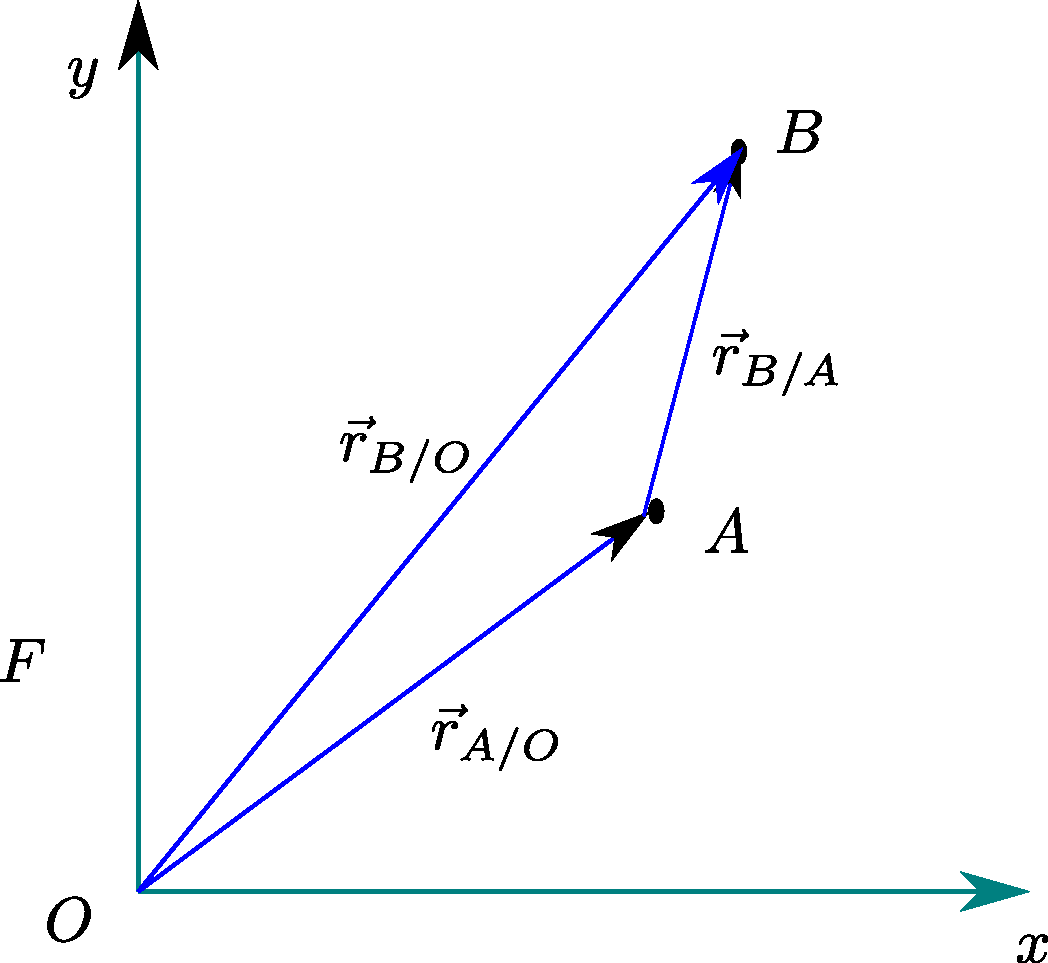
\includegraphics[width=0.6\linewidth]{Bilder/01_DervativeRule.pdf}
	\caption{Geometry of two points using vectors}
	\label{Fig_ch_0_01_DerivateRule}
\end{figure}
The derivative rule gives a mathematical tool for differentiating vectors relative to the frames of reference that they originally do not belong to. The method involves a geometrical approach to differentiating vectors first as described in the following:

Starting from the positions, using the vector formula for addition, we get:
\begin{equation}
	\vec{r}_{B/O} = \vec{r}_{A/O} + \vec{r}_{B/A}
\end{equation}

To find velocities of these, while applying differential operator also note the frames that they are being differentiated:
\begin{equation} \label{Eq_0_ch_0_TT_1}
	\prescript{F}{}{\frac{d \vec{r}_{B/O}}{dt}} = \prescript{F}{}{\frac{d \vec{r}_{A/O}}{dt}} + \prescript{F}{}{\frac{d \vec{r}_{B/A}}{dt}}
\end{equation}
The superscript $F$ applied on the differential operator suggests that differentiation is applied w.r.t frame F. Lets consider first term of equation \eqref{Eq_0_ch_0_TT_1}, this vector as it is referenced directly in frame F and has its tail attached to O, it is directly present in the Frame F and can be therefore, differentiated directly:
\begin{equation}
	\prescript{F}{}{\frac{d \vec{r}_{A/O}}{dt}} = \dot{\vec{r}}_{A/O} = \vec{v}_{A/O}
\end{equation}
For the second term, the tail of the vector is attached to point A which is translating, therefore, vector $\vec{r}_{B/A}$ is not in the Frame F but that of translating Frame A. 
\begin{equation}
	\prescript{F}{}{\frac{d \vec{r}_{B/A}}{dt}} = \prescript{A}{}{\frac{d \vec{r}_{B/A}}{dt}} +   \omega_{} \times \vec{r}_{B/A}
\end{equation} 
This above derivative rule comes into practice due to differentiation of unit vectors that are changing w.r.t to the reference Frame F. The proof of this derivation is as described in the following section.

\subsection{Framing derivative rule for unit vectors}

Consider figure \ref{Fig_0_ch_0_TT_2}. Consider a point P, a position vector an be expressed form O of Frame F. There are two frames in this figure \ref{Fig_0_ch_0_TT_2} with their respective centers and unit vectors as described below
\begin{align*}
	F &: {O,\hat{I},\hat{J},\hat{K}} \\
	B &: {P,\hat{r},\hat{\theta},\hat{k}}
\end{align*}
\begin{figure}[h!]
	\centering
	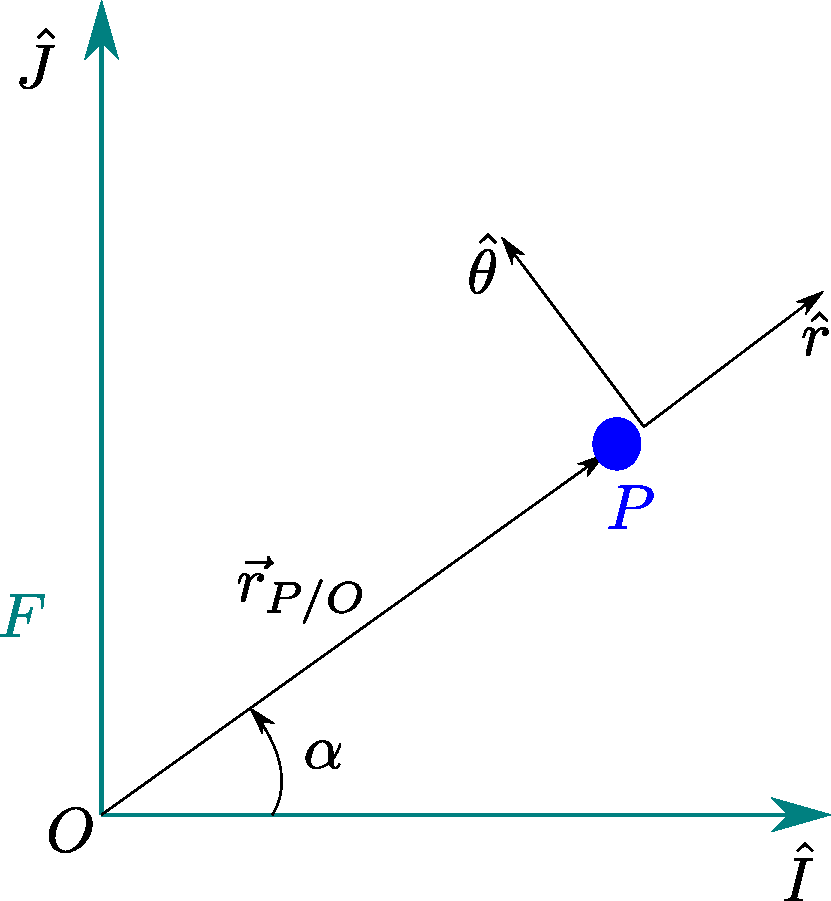
\includegraphics[width=0.5\linewidth]{Bilder/02_derivativeRule_derivation.pdf}
	\caption{Vector of a point represented from body frame to global frame}
	\label{Fig_0_ch_0_TT_2}
\end{figure}
Therefore, using Frame B, the position vector pf point P can be expressed either in body frame as
\begin{equation} \label{Eq_0_ch_0_posVec}
\vec{r}_{P/0} = l \hat{r}
\end{equation}
where $l$ is the length of vector from point O to point P. In order to represent vector $\vec{r}_{P/0}$ on global frame F, consider the rotation of unit vectors as shown in figure \ref{Fig_0_ch_0_TT_3}:
\newpage
\begin{figure}[h!]
	\centering
	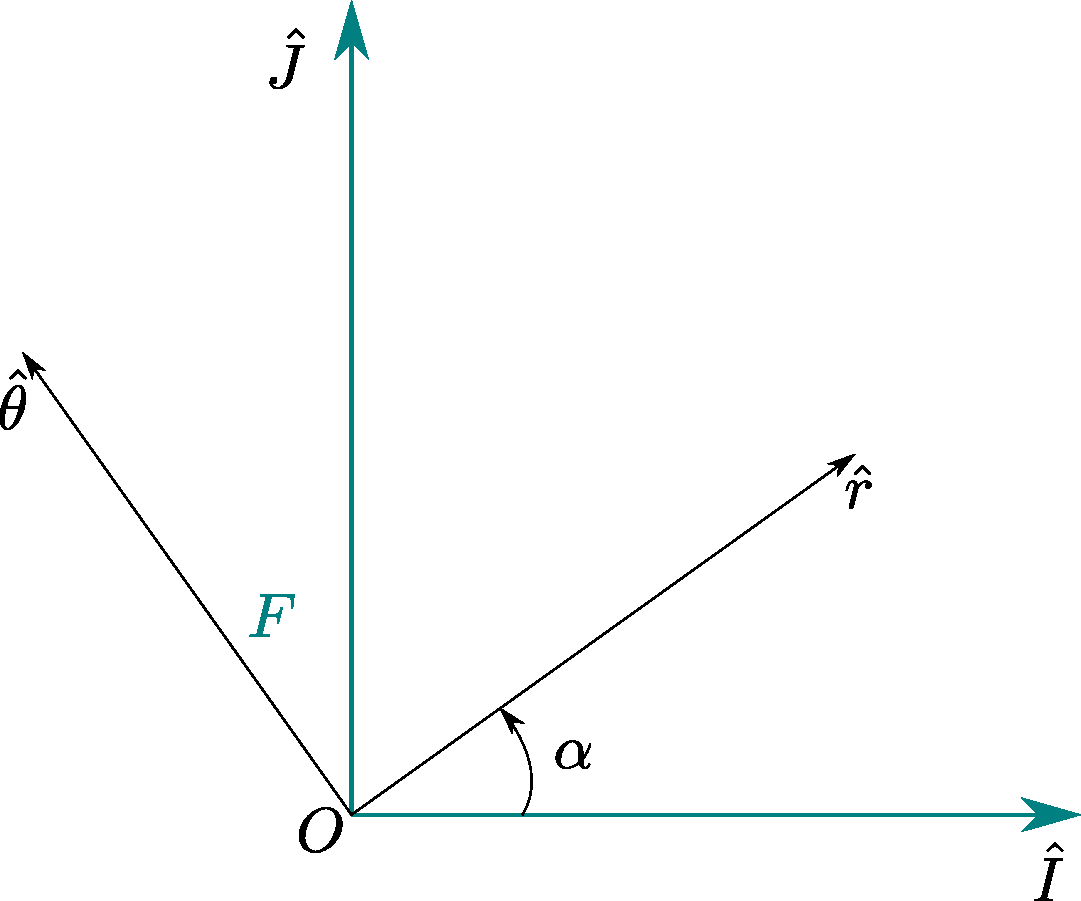
\includegraphics[width=0.5\linewidth]{Bilder/03_UnitVetors_Rotation.pdf}
	\caption{Rotation of unit vectors}
	\label{Fig_0_ch_0_TT_3}
\end{figure}
due to the rotation the unit vectors $\hat{r}$ and $\hat{\theta}$ can be expressed as
\begin{align}
	\hat{r} &= \hat{I}cos\alpha + \hat{J}sin\alpha \\
	\hat{\theta} &= -\hat{I}sin\alpha + \hat{J}cos\alpha
\end{align}
now the velocities of these unit vectors can be determined using differentiation as they have been expressed in frame F as:
\begin{align}
	\prescript{F}{}{\frac{d \hat{r} }{dt}} &= \dot{\hat{r}} = (-sin\alpha \hat{I} + cos\alpha \hat{J})\dot{\alpha} = \dot{\alpha}\hat{\theta} \label{Eq_0_ch_0_TT_4} \\
	\prescript{F}{}{\frac{d \hat{\theta} }{dt}} &= \dot{\hat{\theta}} = (-cos\alpha \hat{I} - sin\alpha \hat{J})\dot{\alpha} = -\dot{\alpha}\hat{r}
\end{align}
therefore, using equation \ref{Eq_0_ch_0_posVec} vector $\vec{r}_{P/0}$ the velocity of this vector can be expressed as:
\begin{equation}
	\prescript{F}{}{\frac{d \vec{r}_{P/0}}{dt}} = \dot{v}_{P/0} = \frac{d l}{dt} \hat{r} + l \frac{d \hat{r}}{dt}
\end{equation}
using equation \eqref{Eq_0_ch_0_TT_4}, we get
\begin{equation}
	\dot{v}_{P/0} = \dot{l} \hat{r} + l \dot{\alpha}\hat{\theta}
\end{equation}
this can further be expressed using cross products between the unit vectors as:
\begin{equation}
\dot{v}_{P/0} = \dot{l} \hat{r} + l \dot{\alpha}(\hat{K} \times \hat{r})
\end{equation}
here the terms $\dot{\alpha}\hat{K}$ is nothing but the angular velocity of Frame B w.r.t Frame F and the term $l \hat{r}$ is nothing but the position vector $\vec{r}_{P/0}$, therefore
\begin{align*}
	\dot{\alpha}\hat{K} &= \omega \\
	l \hat{r} &= \vec{r}_{P/0}
\end{align*}
the velocity equation can now be re-written as
\begin{equation} \label{Eq_0_ch_0_TT}
	\dot{v}_{P/0} = \dot{l} \hat{r} + \omega \times \vec{r}_{P/0}
\end{equation}
the above equation is a used for differentiating vectors in different frames of references. It is also called \textbf{\textit{Transport Theorem}}.

\section{Velocity and Acceleration in moving reference frames}

\subsection{Velocity of a vector in a moving frame}

The transport theorem can be used to determine velocity and acceleration of vector quantities in any moving frames they are attache to. Consider a point B which is attached to a moving reference frame A as shown in figure \ref{Fig_0_ch_0_vecMovingFrames}.
\newpage
\begin{figure}[h!]
	\centering
	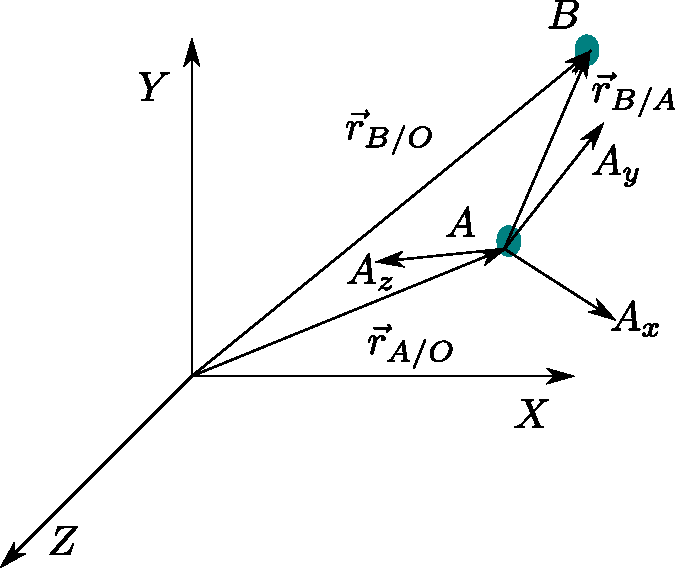
\includegraphics[width=0.55\linewidth]{Bilder/04_vel_acc_movingFrames.pdf}
	\caption{Vectors in moving frames}
	\label{Fig_0_ch_0_vecMovingFrames}
\end{figure}
Assigning frames:
\begin{align*}
	F &: \{ O, \hat{I}, \hat{J}, \hat{K} \}\\
	A &: \{A, \hat{i}, \hat{j}, \hat{k}\}	\\
	B &: \{B, \hat{B_i}, \hat{B_j}, \hat{B_k} \}
\end{align*}
The object is to find velocity and acceleration of vectors of point B that is attached to a moving frame A. Using vector geometry the position of B from O can be determined as:
\begin{equation}
	\vec{r}_{B/O} = \vec{r}_{A/O} + \vec{r}_{B/A}
\end{equation}
for velocities, differentiating the above equation
\begin{align*}
	\prescript{F}{}{\frac{d}{dt}\vec{r}_{B/O}} &= \prescript{F}{}{\frac{d}{dt}\vec{r}_{A/O}} + \prescript{F}{}{\frac{d}{dt}\vec{r}_{B/A}} \\
	\vec{v}_{B/O} &= \vec{v}_{A/O} + \prescript{F}{}{\frac{d}{dt}\vec{r}_{B/A}}
\end{align*}
the term $\vec{v}_{A/O}$ is fixed to the global frame, therefore it is referenced to the unit vectors that are attached to global frame. The second term however, is due to a vector that is attached to a moving frame. This vector needs to be differentiated using transport theorem in order to determine its components properly.

using transport theorem (let point B be described in frame A with position vector $\vec{r}_{B/A} = (Ax \hat{i} + Ay \hat{j} + A_z \hat{k})$ ):
\begin{equation*}
	\prescript{F}{}{\frac{d}{dt}\vec{r}_{B/A}} = \frac{d}{dt}\vec{r}_{B/A} + \omega_{/O} \times \vec{r}_{B/A}
\end{equation*}
therefore, velocity of B which is fixed to a moving reference frame is expressed as:
\begin{equation} \label{Eq_0_ch0_VELwrtMovingFrame}
	v_{B/O} = \vec{v}_{A/O} + \frac{d}{dt}\vec{r}_{B/A} + \omega_{/O} \times \vec{r}_{B/A}
\end{equation}

\textbf{\textit{Note: }}The extra term (third term in equation \eqref{Eq_0_ch0_VELwrtMovingFrame}) is due to differentiating unit vectors of moving frame w.r.t the global frame. The first two terms are literally scalar quantities of the velocities that is, their differentiation does not have any direction associated with them. Just like when energy is differentiated, it is not considered in which frame it is differentiated. Simply a time derivative of these scalar quantities are taken directly. Also, the first two terms of equation \eqref{Eq_0_ch0_VELwrtMovingFrame} are linear velocity of the moving frame itself and the relative velocity of the frame into consideration that is fixed to a moving frame.

\textbf{\textit{Note: }} For all 2D an 3D motion problems the angular velocity term is always chosen to be expressed in the succeeding (frame which is moving compared to the global chosen frame of reference) than the preceding (global frame of reference) frame, mainly because it is always easier to represent $\omega$ in the succeeding frame than the preceding frame for calculation purposes.

In summary, when deriving relative velocity of a vector that is attached to a moving frame has these three following components:
\begin{itemize}
	\item Velocity of the moving frame itself
	\item Velocity of frame in which the vector is being measured (relative to the moving frame)
	\item velocity due ot the rotation of the moving frame w.r.t to the global frame
\end{itemize}

\subsection{Acceleration of a vector in a moving frame}

\begin{equation} \label{Eq_0_ch0_ACCwrtMovingFrame}
	a_{B/O} = \prescript{F}{}{\frac{d}{d}v_{B/O}} = a_{A/O} + \prescript{A}{}{a_{B/A}} + \{ 2 \omega_{/O} \times \prescript{A}{}{v_{B/A}} \} + \{ \dot{\omega}_{/O} \times r_{B/A} \} + \{ \omega_{/O} \times (\omega_{/O} \times r_{B/A}) \}
\end{equation}

in equation \eqref{Eq_0_ch0_ACCwrtMovingFrame}, the following terms are as described
\begin{itemize}
	\item $a_{A/O}$ is due to the acceleration of moving frame itself
	\item $\prescript{A}{}{a_{B/A}} + \{ 2 \omega_{/O} \times \prescript{A}{}{v_{B/A}} \}$ is due to the derivative of second term in equation \eqref{Eq_0_ch0_VELwrtMovingFrame}, where the first term is the relative acceleration of frame B w.r.t frame A, the second term is called Coriolis acceleration and this happens due to a velocity vector that is being rotated by the moving frame. (example of water flowing through channels when these channels are under rotation, the water particles experience Coriolis acceleration)
	\item $ \dot{\omega}_{/O} \times r_{B/A}$ is due to the angular acceleration of moving frame (frame A). Also called Eulerarian acceleration term.
	\item  $\omega_{/O} \times (\omega_{/O} \times r_{B/A})$ is due to the centripetal acceleration (of the form $r \omega^{2}$).
\end{itemize}

\section{Velocity and acceleration w.r.t moving frame in polar coordinates}

Consider figure \ref{Fig_0_ch_0_vel_Acc_polarCoordinates}, this is a 2 DOF problem with rotation about $\hat{k}$ and translation of B on the arm. Consider the following frames in the figure

\begin{figure}[h!]
	\centering
	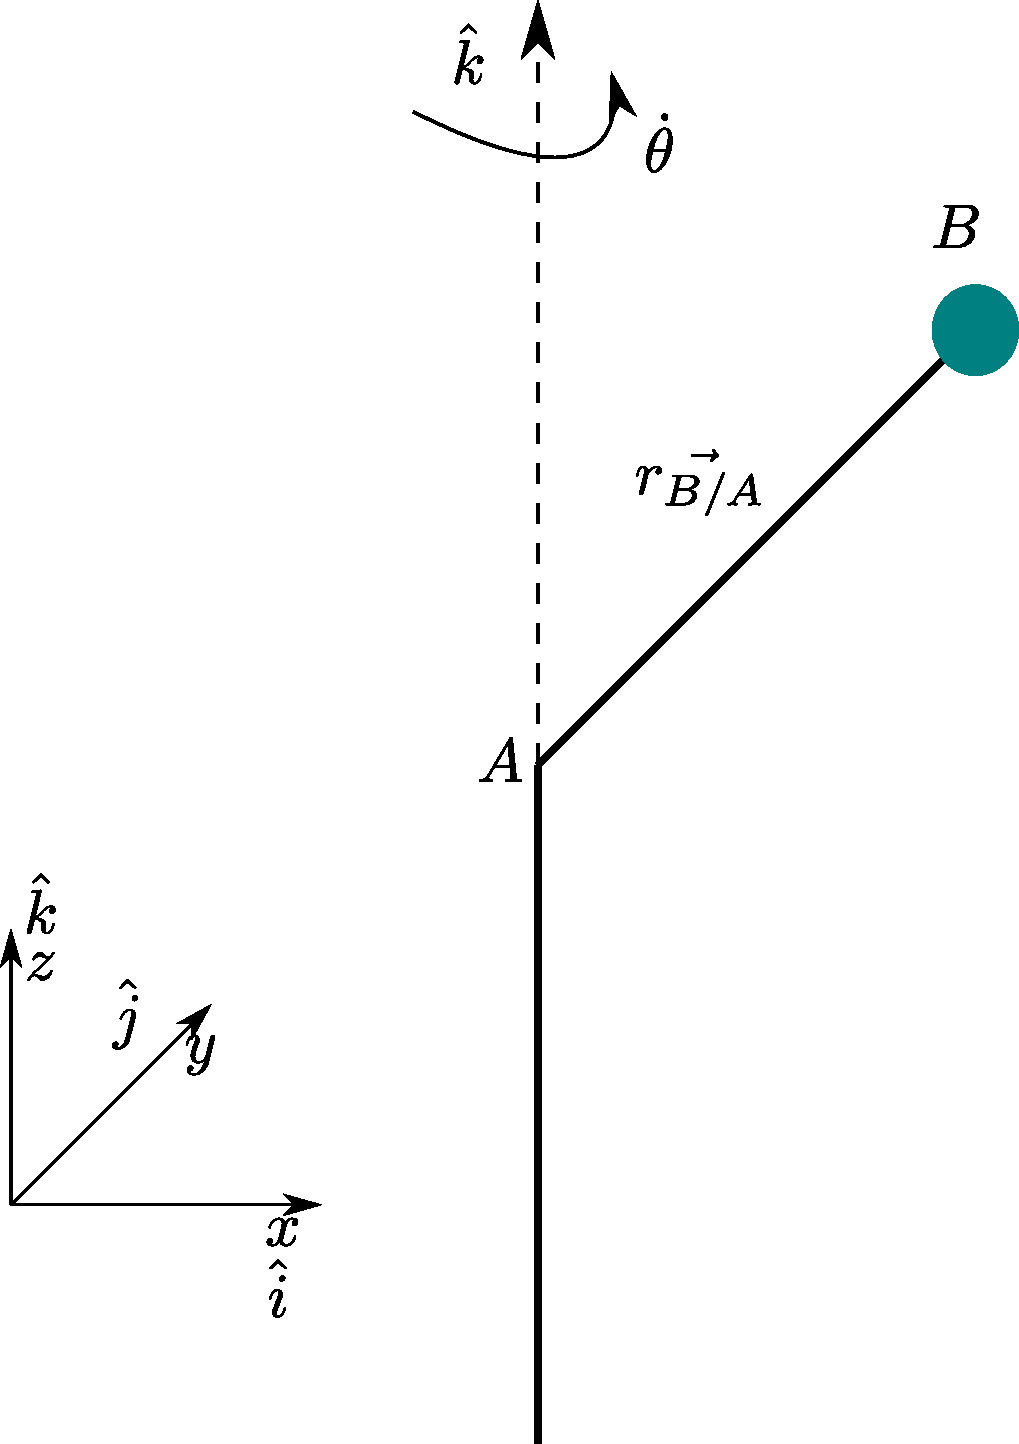
\includegraphics[width=0.5\linewidth]{Bilder/05_vel_acc_polar_coordinates.pdf}
	\caption{2 DOF motion problem stated in polar coordinates}
	\label{Fig_0_ch_0_vel_Acc_polarCoordinates}
\end{figure}

\begin{align*}
	F &: \{O,\hat{i},\hat{j},\hat{k}\} \\
	A &: \{A, \hat{r}, \hat{\theta}, \hat{k}\}
\end{align*}

\newpage
\begin{figure}[h!]
	\centering
	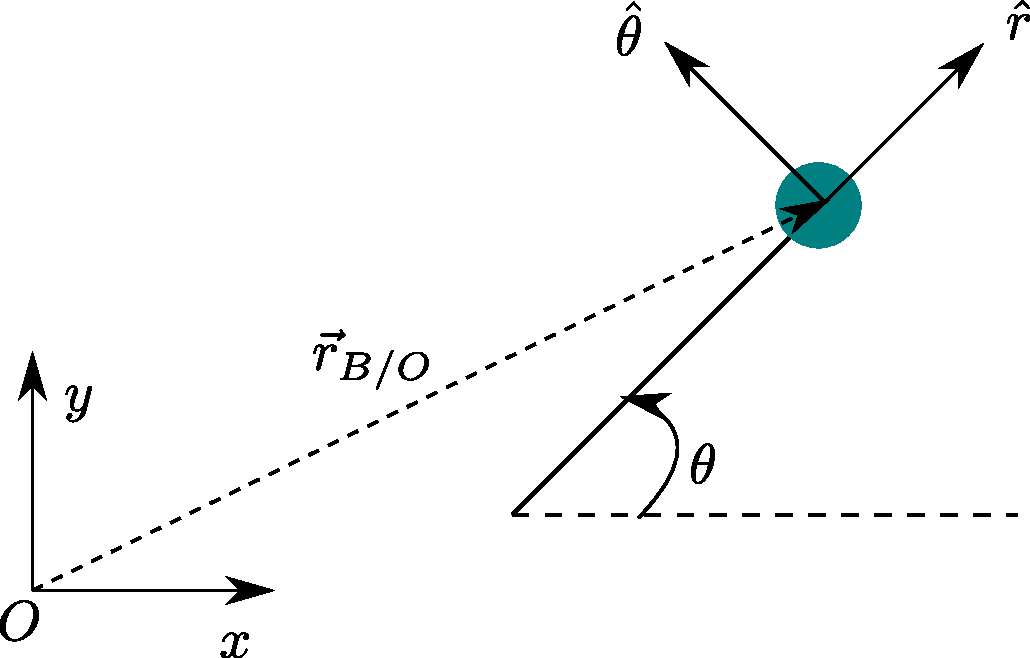
\includegraphics[width=0.5\linewidth]{Bilder/06_vel_acc_polar_coordinates_topView.pdf}
	\caption{Top view of 2 DOF motion problem stated in polar coordinates}
	\label{Fig_0_ch_0_vel_Acc_polarCoordinates_TopView}
\end{figure}

\subsection{Velocity in polar coordinates}

Using the top-view from figure \ref{Fig_0_ch_0_vel_Acc_polarCoordinates_TopView}, the following relations can be derived.
The velocity of point B can be expressed as:
\begin{equation} \label{Eq_0_ch_0_velocityPCD}
	v_{B/O} = v_{A/O} + \prescript{F}{}{\frac{d}{dt}r_{B/A}}
\end{equation}
The acceleration of point B can be expressed as:
\begin{equation} \label{Eq_0_ch_0_accelerationPCD}
	a_{B/O} = a_{A/O}+ \prescript{F}{}{\frac{d^{2}}{dt^{2}}r_{B/A}}
\end{equation}
In general, in rotations problems in 2D, the rotation is about a fixed axis, therefore, $v_{A/O} = a_{A/O} = 0$. This simplification reduces the simple terms from the above equations which can be put back later if needed.

Since this is a 1D rotation problem, the angular velocity can be expressed as:
\begin{equation}
	\omega_{/O} = \dot{\theta}\hat{k}
\end{equation}

From equation \eqref{Eq_0_ch_0_velocityPCD}, using the position vector $r_{B/O} = r \hat{r} + z \hat{k}$:
\begin{equation}
	v_{B/O} = 0 + \prescript{F}{}{\frac{d}{dt}r_{B/A}} = \frac{d}{dt}(r \hat{r} + z \hat{k}) = \dot{r}\hat{r} + r \dot{\hat{r}} + \dot{z}\hat{k} + z \dot{\hat{k}}
\end{equation}
where $\dot{\hat{k}} = 0$, as $\hat{k}$ will never change its direction, therefore, the time derivative of this unit vector is zero. Therefore, the above equation can be re-written as:
\begin{equation}
	v_{B/O} = \dot{r}\hat{r} + r \dot{\hat{r}} + \dot{z}\hat{k}
\end{equation}
there is only one time-derivative of a unit vector that is, $\dot{\hat{r}}$ in this problem. In order to solve for this time-derivative the following figure \ref{fig_0_ch_0_timeDerivativeUnitVector} in considered.
\newpage
\begin{figure}[h!]
	\centering
	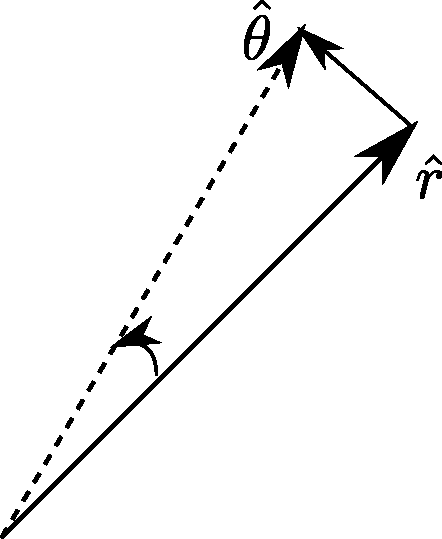
\includegraphics[width=0.25\linewidth]{Bilder/07_UnitVector_Derivative_polar_coordinates.pdf}
	\caption{Taking time-derivative of unit vector in polar coordinates}
	\label{fig_0_ch_0_timeDerivativeUnitVector}
\end{figure}
using this figure \ref{fig_0_ch_0_timeDerivativeUnitVector}, it can be seen that for an infinitesimally small time $\Delta t$, the unit vector $\hat{r}$ moves about an  infinitesimally small length $\dot{\theta}\Delta t$ in the direction of $\hat{\theta}$, therefore:
\begin{equation}
	\Delta \hat{r} = \dot{\theta} \hat{\theta} \Delta t
\end{equation}
where $\Delta \hat{r}$ in figure \ref{fig_0_ch_0_timeDerivativeUnitVector} is the small vector that indicates the change in the direction of this unit vector $\hat{r}$. By re-formulating the above expression, the following can be written:
\begin{equation}
	\frac{\Delta \hat{r}}{\Delta t} = \dot{\theta} \hat{\theta}
\end{equation}
from the above equation, if the limit of $\Delta t$ goes to zero, the expression reaches the definition of a derivative:
\begin{equation}
	\lim_{\Delta t\to 0} \frac{\Delta \hat{r}}{\Delta t} = \frac{d}{dt}\hat{r} = \dot{\theta} \hat{\theta}
\end{equation}
therefore, deriving the time derivative of the required unit vector. The velocity of B in polar coordinates can therefore be expressed as (including velocity of the moving frame itself):
\begin{equation}
	v_{B/O} = v_{A/O} + \dot{r}\hat{r} + r \dot{\theta} \hat{\theta} + \dot{z}\hat{k}
\end{equation}
The above expression for velocity in polar coordinates can simply be determined using Transport Theorem, without getting into the details of polar coordinates themselves as described below. Using equation \eqref{Eq_0_ch_0_velocityPCD}
\begin{equation}
	\prescript{F}{}{\frac{d}{dt}r_{B/O}} = \prescript{A}{}{\frac{d}{dt}r_{B/A}} + \omega_{/O} \times r_{B/A}
\end{equation}
substituting for $r_{B/A}$ in the above equation:
\begin{align*}
	\prescript{F}{}{\frac{d}{dt}r_{B/O}} &= \prescript{A}{}{\frac{d}{dt}}(r \hat{r} + z \hat{k}) + \omega_{/O} \times r \hat{r} + z \hat{k} \\
	\prescript{F}{}{\frac{d}{dt}r_{B/O}} &= \dot{r}\hat{r} + \dot{z}\hat{k} + \dot{\theta}\hat{k} \times (r \hat{r} + z \hat{k}) \\
	\prescript{F}{}{\frac{d}{dt}r_{B/O}} &= \dot{r}\hat{r} + \dot{z}\hat{k} + r \dot{\theta} \hat{\theta}
\end{align*}

\subsection{Acceleration in polar coordinates}

From equation \eqref{Eq_0_ch_0_accelerationPCD}, acceleration is expressed as:
\begin{equation}
	a_{B/O} = a_{A/O}+ \prescript{F}{}{\frac{d^{2}}{dt^{2}}r_{B/A}} = 0 + \prescript{F}{}{\frac{d}{dt}v_{B/A}} = \frac{d}{dt}(\dot{r}\hat{r} + \dot{z}\hat{k} + r \dot{\theta} \hat{\theta})
\end{equation}
simplifying the above expression:
\begin{align*}
	a_{B/O} &= \ddot{r}\hat{r} + \dot{r}\dot{\hat{r}} + \ddot{z}\hat{k} + \dot{z}\dot{\hat{k}} + \dot{r}\dot{\theta} \hat{\theta} + r \ddot{\theta} \hat{\theta} + r \dot{\theta} \dot{\hat{\theta}} \\
	a_{B/O} &= \ddot{r}\hat{r} + \dot{r} \dot{\theta} \hat{\theta} + \ddot{z}\hat{k} + 0 + \dot{r}\dot{\theta} \hat{\theta} + r \ddot{\theta} \hat{\theta} - r \dot{\theta}^{2} \hat{r}
\end{align*}
therefore, the acceleration in polar coordinates including $a_{A/O}$ can be expressed as:
\begin{equation} \label{Eq_accelrationInPolarCoordinates}
	a_{B/O} = a_{A/O} + (\ddot{r}\hat{r} + \ddot{z}\hat{k}) + 2 \dot{r} \dot{\theta} \hat{\theta} +  r \ddot{\theta} \hat{\theta} - r \dot{\theta}^{2} \hat{r}
\end{equation}
where
\begin{itemize}
	\item $a_{A/O}$ acceleration of the moving frame itself
	\item $(\ddot{r}\hat{r} + \ddot{z}\hat{k})$ relative acceleration of a moving point B which is connected to moving frame A
	\item $2 \dot{r} \dot{\theta} \hat{\theta}$ is the Coriolis acceleration
	\item $r \ddot{\theta} \hat{\theta}$ is Euler's acceleration due to $\ddot{\theta}$
	\item $r \dot{\theta}^{2} \hat{r}$ is the centripetal (or centrifugal acceleration)
\end{itemize}

\textbf{\textit{Note: }} The same exact method is employed while deriving expressions for 3D dynamics problems both in Cartesian and polar coordinates.

\section{Rotation Problem 1}

Consider a 1D rotation problem as shown in figure \ref{Fig_Rotation_Problem_1}. Consider the following frames
\newpage
\begin{figure}[h!]
	\centering
	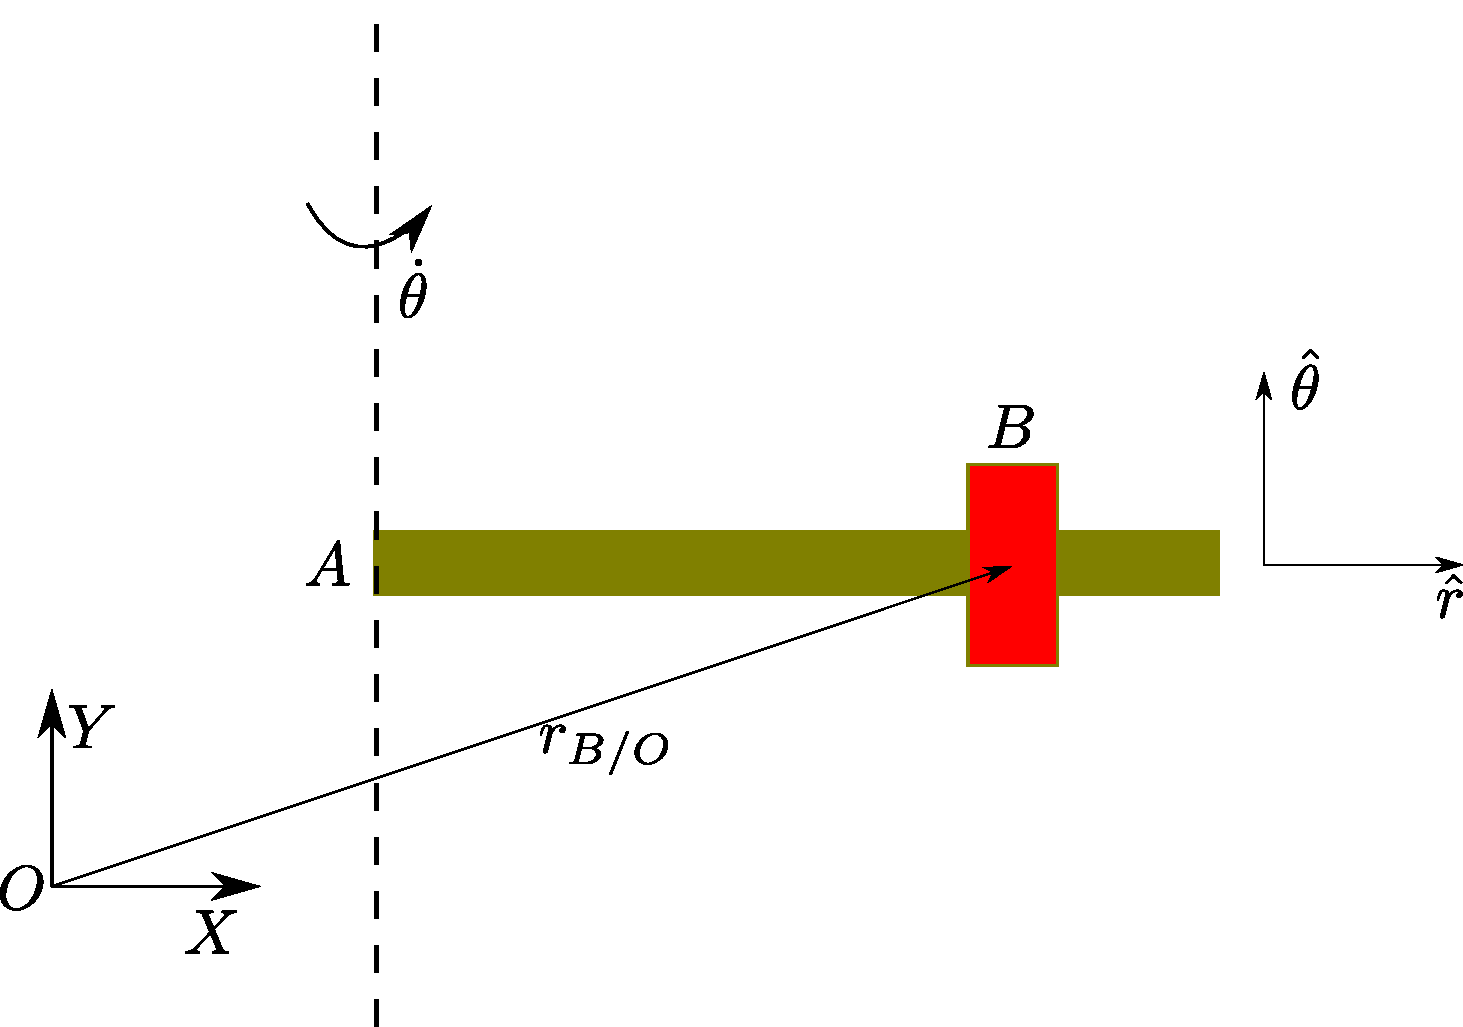
\includegraphics[width=0.65\linewidth]{Bilder/08_RotationProblem1.pdf}
	\caption{Rotation Problem 1}
	\label{Fig_Rotation_Problem_1}
\end{figure} 
\begin{align*}
	F &: \{O, X (\hat{i}), Y (\hat{j}), Z (\hat{k})\} \\
	A &: \{A, \hat{r}, \hat{\theta}, \hat{k}\}
\end{align*}
Frame O is the inertial reference frame, A is the moving frame w.r.t Frame O. The green bar is a pipe which is rotating at a speed $\omega_{/O} = \dot{\theta}\hat{k}$. B is a nut which is constrained to moving along the green bar at a constant velocity $\dot{r}\hat{r}$. The object is to find the velocity and acceleration of B $r_{B/O}$.

In order to solve this problem, consider the velocity formula in polar coordinates (consider polar coordinates while solving problems related to 1D rotation).
\begin{equation}
	v_{B/O} = v_{A/O} + \dot{r}\hat{r} + r \dot{\theta} \hat{\theta} + \dot{z}\hat{k}
\end{equation}
in the above equation $v_{A/O} = 0$ as well as $\dot{z}\hat{k} = 0$ as this problem is constrained only to 1D rotation and 1D translation $\dot{r}\hat{r}$. Therefore, reducing the velocity to the following terms:
\begin{equation}
	v_{B/O} = \dot{r}\hat{r} + r \dot{\theta} \hat{\theta}
\end{equation}
For acceleration, consider the acceleration equation in polar coordinates:
\begin{equation}
a_{B/O} = a_{A/O} + (\ddot{r}\hat{r} + \ddot{z}\hat{k}) + 2 \dot{r} \dot{\theta} \hat{\theta} +  r \ddot{\theta} \hat{\theta} - r \dot{\theta}^{2} \hat{r}
\end{equation}
where $a_{A/O} = 0$, $(\ddot{r}\hat{r} + \ddot{z}\hat{k}) = 0$ and $r \ddot{\theta} \hat{\theta} = 0$, therefore reducing the above equation to:
\begin{equation}
	a_{B/O} = 2 \dot{r} \dot{\theta} \hat{\theta} - r \dot{\theta}^{2} \hat{r}
\end{equation}
Now, its all about finding the forces using Newton's second law $\sum F_{ext} = m a_{B/O}$
\begin{align}
	\sum F_{ext} \hat{r} &= m a_{B/O} \cdot \hat{r} = - m r \dot{\theta}^{2} \hat{r} \\
	\sum F_{ext} \hat{\theta} &= m a_{B/O} \cdot \hat{\theta} = 2 m \dot{r} \dot{\theta} \hat{\theta}
\end{align}
here, $- m r \dot{\theta}^{2} \hat{r}$ is the centripetal force, this is a necessary force that is required to maintain a circular motion. The other force $2 m \dot{r} \dot{\theta} \hat{\theta}$ is a Coriolis force, the existence of this force can be explained using \textbf{\textit{law of conservation of momentum}}.

\subsection{Explaining Coriolis force using Law of conservation of angular momentum}

Using the definition of angular momentum, we get:
\begin{equation}
	h_{B/O} = r_{B/O} \times p_{B/O} = r_{B/O} \times m v_{B/O}
\end{equation}
\begin{equation}
	h_{B/O} = r \hat{r} \times ( m \dot{r}\hat{r} + r \dot{\theta} \hat{\theta}) = m r^{2} \dot{\theta} \hat{k}
\end{equation}
torque is defined as the time-derivative of angular momentum:
\begin{equation}
	\frac{d}{dt}h_{B/O} = 2 m r \dot{r} \dot{\theta} \hat{k} = r_{B/O} \times F_{cor}
\end{equation}
it can be seen that the $F_{cor}$ term in the above equation is nothing but the term $2 m \dot{r} \dot{\theta} \hat{\theta}$ from equation of $\sum F_{ext} \hat{\theta}$. Therefore, this Coriolis force is the force that comes into action when a particle / body in translation is also under rotation due to the frame that it is fixed to. Similar to centripetal force, Coriolis force is also a necessary force that is required to conserve the angular momentum in case of problems concerning 1D rotation with 1D translation to it.

\section{Rotation Problem 2}

Consider a problem as shown in figure \ref{Fig_RotationProblem_2}. Unlike problem 1, the nut is here replaced with a ball that is not constrained so additionally we have $\ddot{r}$, ie., the ball can accelerate due to the rotation of the pipe as it is no more constrained by the centripetal acceleration. the arrow pointing out of the ball is the velocity $\dot{r}$ along $\hat{r}$ direction.
\newpage
\begin{figure}[h!]
	\centering
	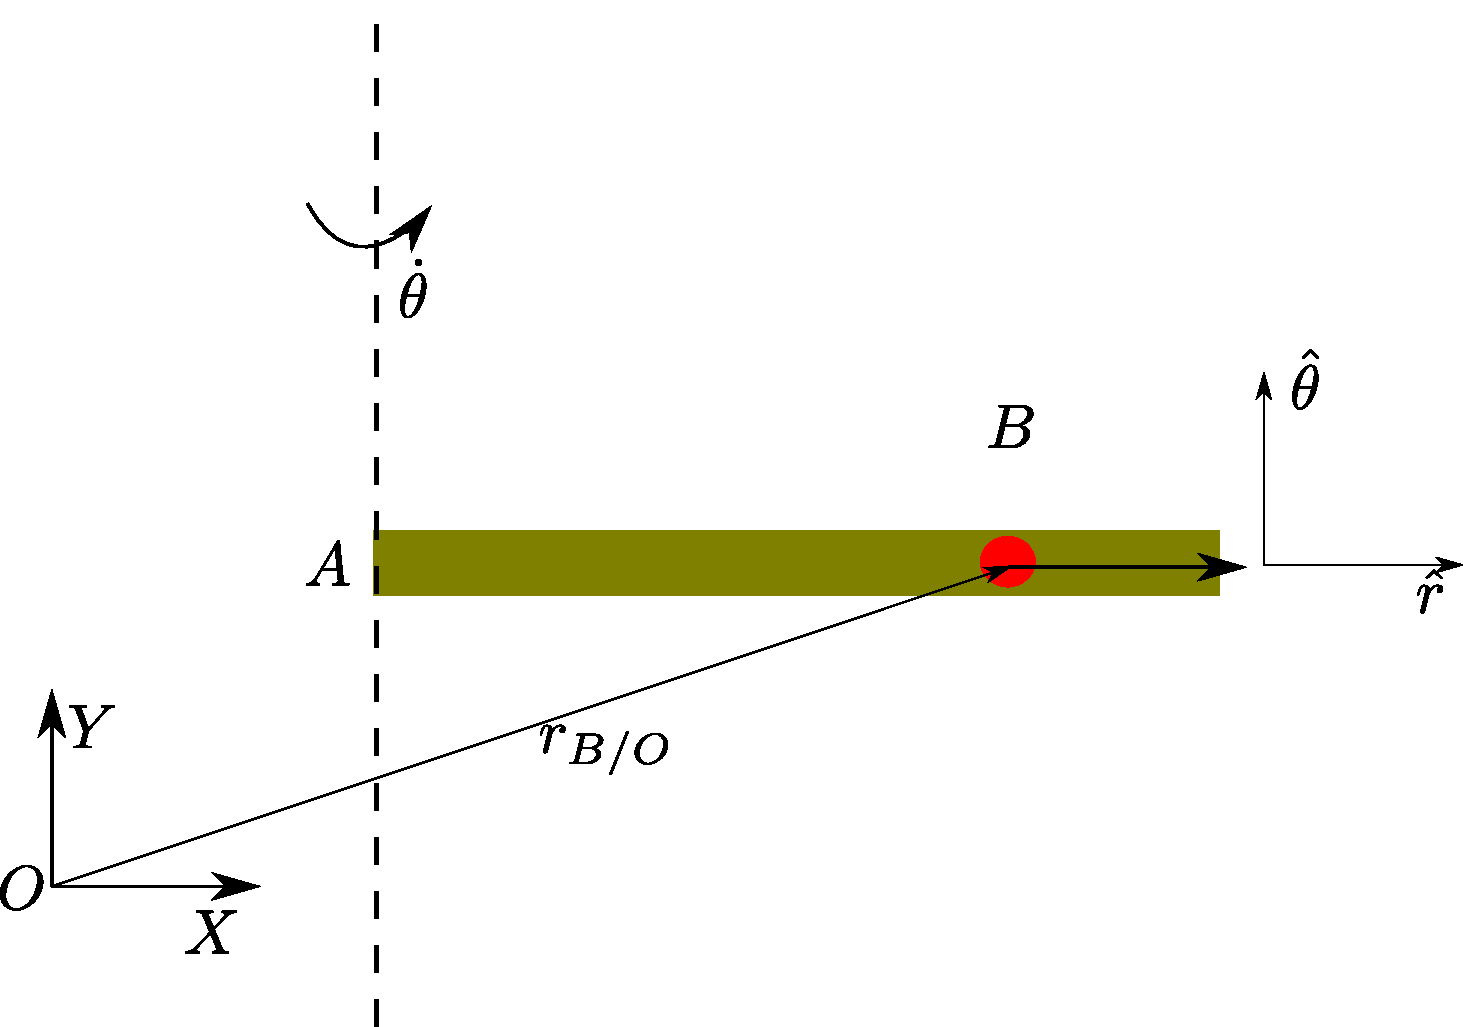
\includegraphics[width=0.65\linewidth]{Bilder/08_RotationProblem2.pdf}
	\caption{Rotation problem 2}
	\label{Fig_RotationProblem_2}
\end{figure}
applying velocity formula for the polar coordinates:
\begin{equation}
	v_{B/O} = \dot{r}\hat{r} + r \dot{\theta} \hat{\theta}
\end{equation}
acceleration:
\begin{equation}
	a_{B/0} = \ddot{r}\hat{r} + 2 \dot{r} \dot{\theta} \hat{\theta} +  r \ddot{\theta} \hat{\theta} - r \dot{\theta}^{2} \hat{r}
\end{equation}
The forces acting on the ball along the two directions are:
\begin{align}
	\sum F_{\hat{r}} &= m (\ddot{r} - r \dot{\theta}^{2}) \hat{r} \\
	\sum F_{\hat{\theta}} &= m (2 \dot{r} \dot{\theta} + r \ddot{\theta})\hat{\theta}
\end{align}
consider $\sum F_{\hat{r}}$, it can be seen that since $m \neq 0$, the expression follows as $\ddot{r} = r \dot{\theta}^{2}$. So basically, the acceleration along the $\hat{r}$ direction is equal to the centripetal acceleration. In other words, in absence of centripetal acceleration, the ball will now accelerate by a quantity of $r \dot{\theta}^{2}$. Which means that $r \dot{\theta}^{2}$ is the required centripetal acceleration if the ball is supposed to be constrained to move along a circular path. Therefore, centripetal acceleration is a necessary condition for an object that is moving along a circular path.

\section{Rotation Problem 3}

Consider figure \ref{Fig_RotationProblem3}.
\newpage
\begin{figure}[h!]
	\centering
	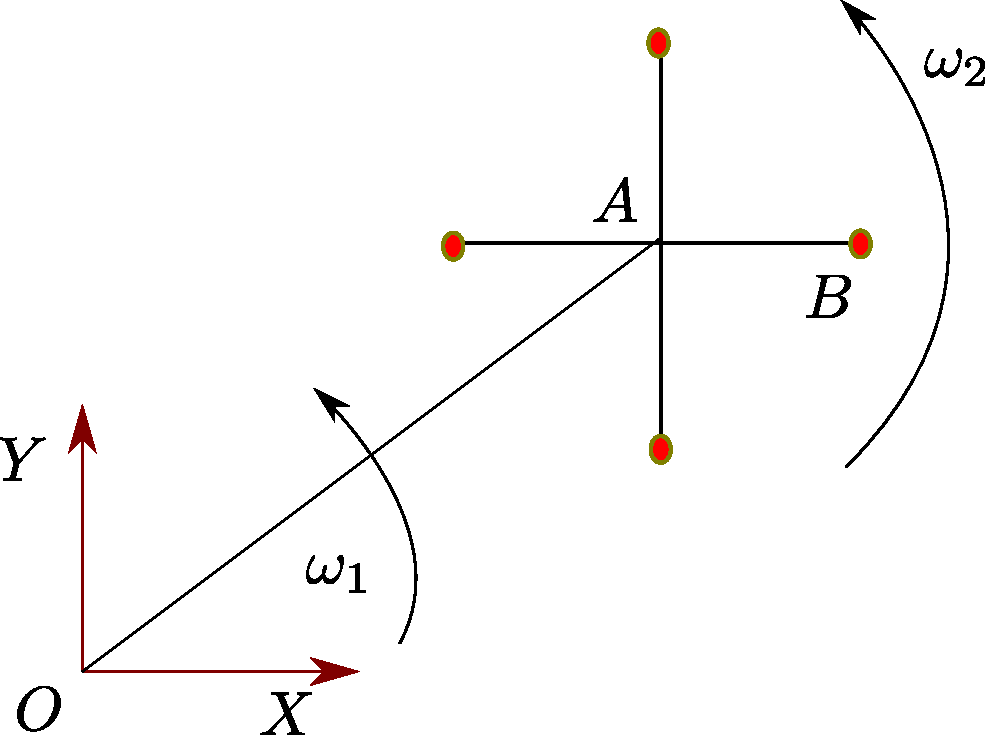
\includegraphics[width=0.65\linewidth]{Bilder/08_RotationProblem3.pdf}
	\caption{Rotation Problem 3}
	\label{Fig_RotationProblem3}
\end{figure}

Frames:
\begin{align*}
	F &: \{ O, \hat{i_{1}}, \hat{j_{1}}, \hat{k_{1}} \} \\
	arm &: \{ c, \hat{i_{2}}, \hat{j_{2}}, \hat{k_{2}} \} \\
	A &: \{ A, \hat{i_{3}}, \hat{j_{3}}, \hat{k_{3}} \} \\
\end{align*}

Angular velocity of B w.r.t A:
\begin{equation}
	\omega_{B/O} = (\omega_{2} + \omega_{1}) \hat{k}
\end{equation}
velocity:
\begin{equation}
	v_{B/O} = v_{A/O} + v_{B/A} + \omega_{B/O} \times r_{B/A}
\end{equation}
further determining $v_{A/O}$: (Not shown in the diagram A is the center of the rotation spokes, but the arm to which A is fixed has its own frame, lets call this frame center as c and let it coincide with point O). Let R be the arm length:
\begin{equation}
	v_{A/O} = v_{c/O} + v_{A/c} + \omega_{1}\hat{k_{1}} \times r_{A/c} = 0 + 0 + \omega_{1}\hat{k_{1}} \times R \hat{i_{1}} = R \omega_{1} \hat{j_{1}}
\end{equation}
simplifying the above equation
\begin{equation}
	v_{B/O} = 0 + R \omega_{1} \hat{j_{1}} + (\omega_{2} + \omega_{1}) \hat{k} \times l \hat{i_{2}} = R \omega_{1} \hat{j_{1}} + l (\omega_{2} + \omega_{1}) \hat{j_{2}}
\end{equation}

\section{Derivative on angular velocity $\omega$}

Consider figure \ref{fig_0_ch_0_omegawithZerotiltAngle}. The axis-y of both the wheel and the cross are aligned with zero angle between them. 
\begin{figure}[h!]
	\centering
	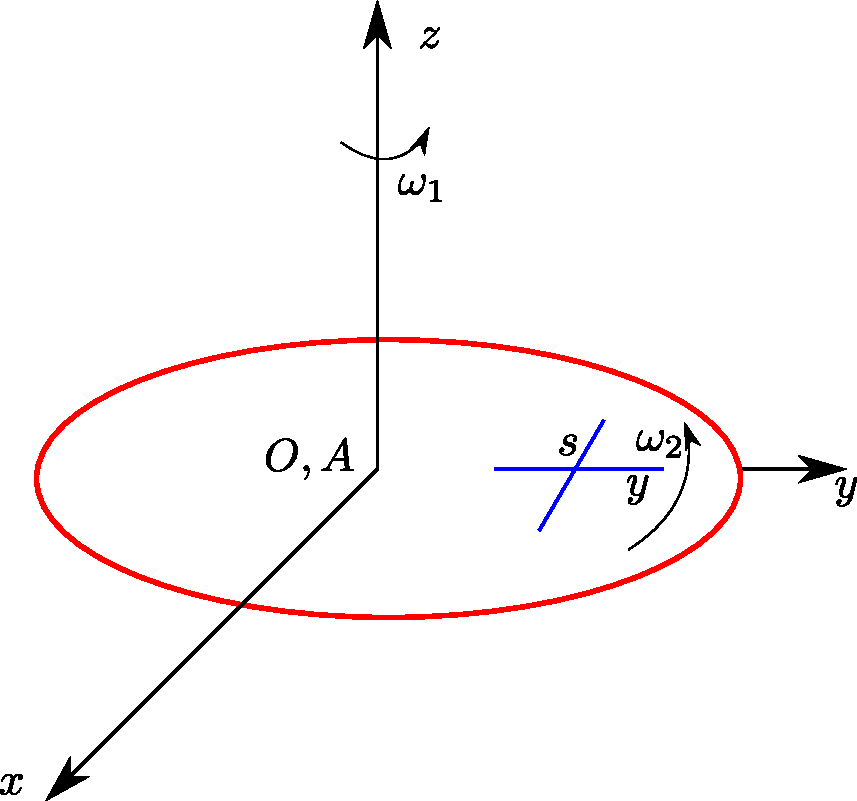
\includegraphics[width=0.5\linewidth]{Bilder/14_timeDerivativeAngVeocity.pdf}
	\caption{Anglar velocity with zero tilt angle}
	\label{fig_0_ch_0_omegawithZerotiltAngle}
\end{figure}

In such a case, in order to find the angular velocity of $s$, both $\omega_{1}$ and $\omega_{2}$ can be added directly, as $\omega$ is a vector and a linear operation is possible.

\textbf{\textit{Note: }}This is not possible with angles as they are not vectors and need to be added up using DCM's or related methods using DCM's such as Euler angles.

Let the frames of the wheel and the cross be respectively as follows:
\begin{align*}
	F &:\{ O, \hat{I}, \hat{J}, \hat{K} \} \\
	C &:\{ A, \hat{i}, \hat{j}, \hat{k} \}
\end{align*}

The angular velocity $\omega_{s}$ is expressed using addition theorem (not covered in this book):
\begin{equation}
	\omega_{s} = \omega_{2} \hat{j} + \omega_{1}\hat{I}
\end{equation}

\textbf{\textit{Note: }} Care should be taken to do time-derivative on any vectors that belong to $s$ as $s$ is attached to a moving frame $F$.

differentiating above equation w.r.t frame F:
\begin{equation} \label{Eq_0_ch_0_omegaDot2}
	\prescript{F}{}{\frac{d}{dt}\omega_{s}} = \dot{\omega_{s}} = \frac{d}{dt}\left( \omega_{2} \hat{j} \right) + \frac{d}{dt}\left( \omega_{1}\hat{K} \right)
\end{equation}
where
\begin{itemize}
	\item $\frac{d}{dt}\left( \omega_{2} \hat{j} \right)$ can be obtained using transport theorem as this is a vector attached to a moving frame A
	\item $\frac{d}{dt}\left( \omega_{1}\hat{K} \right) = \dot{\omega_{1}}\hat{K}$, as derivative of $\hat{K}$ w.r.t frame F will be zero
\end{itemize}
further using transport theorem:
\begin{equation} \label{Eq_0_ch_0_omegaDot1}
	\frac{d}{dt}\left( \omega_{2} \hat{j} \right) = \dot{\omega}_{2}\hat{j} + \omega_{1}\hat{K} \times \omega_{2} \hat{j} = \dot{\omega}_{2}\hat{j} - \omega_{1}\omega_{2}\hat{i}
\end{equation}

\textbf{\textit{Note: }} Transport theorem (TT) works this way, the first term in TT is the term which has time derivative of a scalar (i.e., only a quantity) with no rotations associated with it (therefore, no unit vectors derivative) and a second term due to rotations (where unit vectors are time-differentiated), therefore, associating (unit vectors) with the rotation vector.

since unit vectors $\hat{K}$ and $\hat{k}$ are aligned, the above cross-product can be performed directly.

using equation \eqref{Eq_0_ch_0_omegaDot1} in equation \ref{Eq_0_ch_0_omegaDot2}, we get:
\begin{equation}
	\dot{\omega_{s}} = \dot{\omega}_{2}\hat{j} - \omega_{1}\omega_{2}\hat{i} + \dot{\omega_{1}}\hat{K}
\end{equation}

